\section{Лекция 5.12.2019}


\subsection{Размерность подпространства конечномерного векторного пространства}

Пусть $V$ -- конечномерное векторное пространство.

\begin{proposal}
    Если $U \subseteq V$ -- подпространство $V$, тогда $U$ тоже конечномерно, причем $\dim U \leq \dim V$. 

    Кроме того, $\dim U = \dim V \iff U = V$.
\end{proposal}

\begin{proof}
    Пусть $n = \dim V$.

    Построим в $U$ конечный базис.

    Если $U = \{\overrightarrow{0}\}$, то в качестве базиса берем $\varnothing$.

    Далее считаем, что $U \neq \{\overrightarrow{0}\}$. 

    Выберем $v_1 \in U \setminus \{\overrightarrow{0}\}$. Если $\langle v_1 \rangle = U$, то конец. Иначе, выберем $v_2 \in U \setminus \langle v_1 \rangle$.

    Если $\langle v_1, v_2 \rangle = U$, то конец.

    Иначе, выберем $v_3 \in U \setminus \langle v_1, v_2 \rangle$, и так далее.

    Получаем систему векторов $v_1, v_2, \dots$. Она линейно независима по \hyperref[lec12:lemma]{лемме}.

    \bigskip
    По \hyperref[lec11:osnovnaya_lemma_o_lin_zavisimosti]{основной лемме о линейной зависимости} процесс закончится не позднее шага $n$, значит $U$ конечномерно и $\dim U \leq \dim V$.

    Если $\dim U = n$, то $v_1, \dots, v_n$ -- базис $U$. 
    По следствию, если $v_1, \dots, v_n$ -- базис $U$, то $U = V$.
\end{proof}


\subsection{Ранг системы векторов}

Пусть $\dim V < \infty$ и $S \subseteq V$ -- система векторов.

\begin{definition}
    \textit{Рангом} системы векторов $S$  называется число $\rk S$, равное наибольшему числу векторов в линейно независимой подсистеме из $S$.
    \begin{equation*}
        \rk S = \max \{|S'| \mid S' \subseteq S \text{ -- линейно независимая подсистема}\}
    .\end{equation*}
\end{definition}


\subsection{Связь ранга системы векторов с размерностью её линейной оболочки}

\begin{proposal}
    $\rk S = \dim \langle S \rangle$.
\end{proposal}

\begin{proof}
    Пусть $\rk S = r$.

    Тогда существует линейно независимая подсистема $S' = \{v_1, \dots, v_r\}$.

    По определению ранга и лемме получаем $S \subseteq \langle v_1, \dots, v_r \rangle$.

    Значит, $\langle S \rangle = \langle v_1, \dots, v_r \rangle$ (так как $v_1, \dots, v_r \in S$).

    Следовательно $\dim S = r$.
\end{proof}


\subsection{Ранг матрицы: столбцовый и строковый}

Пусть $A \in \text{Mat}_{m \times n}(F)$.

\begin{definition}
    \textit{Столбцовым рангом} (или просто \textit{рангом}) матрицы $A$ называется ранг системы её столбцов
    \begin{equation*}
        A^{(1)}, \dots, A^{(n)} \subseteq F^{n}
    .\end{equation*}

    Обозначение: $\rk A = \rk \{A^{(1)}, \dots, A^{(n)}\}$.
\end{definition}

\begin{definition}
    \textit{Строковым рангом} матрицы $A$ называется число $\rk A^T$, то есть ранг системы строк
    \begin{equation*}
        A_{(1)}, \dots, A_{(n)} \in F^n
    .\end{equation*}
\end{definition}

\begin{example}
    \begin{equation*}
        A = \begin{pmatrix} 1 & 2 & 3 \\ 4 & 5 & 6 \\ 7 & 8 & 9 \end{pmatrix} 
    \end{equation*}
    
    Любые два столбца линейно независимы (не пропорциональны), то есть $\rk A \geq 2$.

    Но, $A^{(2)} = \frac{1}{2}\left(A^{(1)} + A^{(3)}\right)$, значит $A^{(1)}, A^{(2)}, A^{(3)}$ линейно зависимы $\implies \rk A = 2$.
\end{example}


\subsection{Сохранение линейных зависимостей между столбцами матрицы при элементарных преобразованиях строк}

\begin{proposal}
    Элементарные преобразования строк сохраняют линейные зависимости между столбцами матрицы.

    Если $A \rightsquigarrow B$ элементарным преобразованиями строк, то
    \begin{equation*}
        \alpha_1 A^{(1)} + \dots + \alpha_n A^{(n)} = \overrightarrow{0}
        \iff
        \alpha_1 B^{(1)} + \dots + \alpha_n B^{(n)} = \overrightarrow{0}
    .\end{equation*}

    В частности, при $1  \leq i_1 < \dots < i_k \leq n$
    \begin{equation*}
        A^{(i_1)}, \dots, A^{(i_k)} \text{ линейно независимы}
        \iff
        B^{(i_1)}, \dots, B^{(i_k)} \text{ линейно независимы}
    .\end{equation*}
\end{proposal}

\begin{proof}
    \begin{align*}
        \alpha_1 A^{(1)} + \dots + \alpha_n A^{(n)} = \overrightarrow{0}
        &\iff
        A \cdot \begin{pmatrix} \alpha_1 \\ \dots \\ \alpha_n \end{pmatrix} = \overrightarrow{0}
        \\ &\iff 
        \begin{pmatrix} \alpha_1 \\ \dots \\ \alpha_n \end{pmatrix} \text{ --- решение ОСЛУ } Ax = \overrightarrow{0}
        \\ &\iff
        \begin{pmatrix} \alpha_1 \\ \dots \\ \alpha_n \end{pmatrix} \text{ --- решение ОСЛУ } Bx = \overrightarrow{0}
        \\ &\iff
        B \cdot \begin{pmatrix} \alpha_1 \\ \dots \\ \alpha_n \end{pmatrix} = \overrightarrow{0}
        \iff
        \alpha_1 B^{(1)} + \dots + \alpha_n B^{(n)} = \overrightarrow{0}
        \qedhere
    .\end{align*}
\end{proof}


\subsection{Инвариантность столбцового и строкового рангов матрицы при элементарных преобразованиях строк и столбцов}

\begin{corollary}
    При элементарных преобразованиях строк (столбцовый) ранг матрицы сохраняется.
\end{corollary}

\begin{proposal}
    При элементарных преобразованиях столбцов линейная оболочка $\langle A^{(1)}, \dots, A^{(n)} \rangle$ сохраняется.
\end{proposal}

\begin{proof}
    Пусть $A \rightsquigarrow B$ элементарными преобразованиями столбцов.

    Тогда, 
    \begin{equation*}
        B^{(1)}, \dots, B^{(n)} \in \langle A^{(1)}, \dots, A^{(n)} \rangle
    .\end{equation*}

    Значит, 
    \begin{equation*}
        \langle B^{(1)}, \dots, B^{(n)} \rangle \subseteq \langle A^{(1)}, \dots, A^{(n)} \rangle
    .\end{equation*}

    Так как элементарные преобразования обратимы, то включение верно и в другую сторону.
\end{proof}

\begin{corollary}
    При элементарных преобразованиях столбцов (столбцовый) ранг матрицы сохраняется.
\end{corollary}

\begin{corollary}
    Строковый ранг матрицы сохраняется при элементарных преобразованиях строк и столбцов.
\end{corollary}


\subsection{Столбцовый и строковый ранги матрицы, имеющей улучшенный ступенчатый вид}

\begin{proposal}
    Если $A$ имеет улучшенный ступенчатый вид, то оба числа $\rk A$ и $\rk A^T$ равны числу ненулевых строк~в~$A$.
\end{proposal}

\begin{proof}
    Пусть $r$ -- число ненулевых строк в $A$ и пусть $i_1 < \dots < i_r$ -- номера ведущих элементов строк.
    \begin{center}
        \begin{math}
            \bordermatrix{
                  & & & & i_1 & & i_2 & & i_3 & & i_r & \cr
                  & 0 & \dots & 0 & 1 & & 0 & & 0 & & 0 & \cr
                  &   &   &   & 0 & \dots & 1 & & 0 & & \vdots & \cr
                  &   &   &   & \vdots &   & 0 & \dots & 1 &   & 0 & \cr
                  &   &   &   & \vdots & & \vdots &   & 0 & \dots & 1 & \cr
                  &   &   &   & 0 &   & 0 &   & 0 &   & 0 & \cr
            }
            \hspace{1cm}
            \vcenter{\hbox{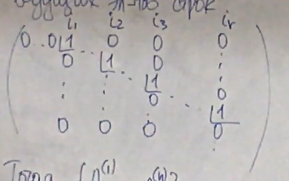
\includegraphics[scale=0.5]{img/lecture13_matrix.png}}}
        \end{math}

        \tiny жалкая попытка повторить шедевр
    \end{center}

    Тогда, $\{A^{(1)}, \dots, A^{(n)}\} \ni e_1, \dots, e_r$, где 
    \begin{equation*}
        e_i = \begin{pmatrix} 0 \\ \dots \\ 0 \\ 1 \\ 0 \\ \dots \\ 0 \end{pmatrix} \leftarrow i
    .\end{equation*}

    Значит, $\langle A^{(1)}, \dots, A^{(n)} \rangle \supseteq \langle e_1, \dots, e_r \rangle$.

    Заметим, что $A^{(1)}, \dots, A^{(n)} \in \langle e_1, \dots, e_r \rangle$, то есть $\langle A^{(1)}, \dots, A^{(n)} \rangle \subseteq \langle e_1, \dots, e_r \rangle$.

    \bigskip
    Теперь покажем, что строки $A_{(1)}, \dots, A_{(r)}$ линейно независимы.

    Пусть $\alpha_1 A_{(1)} + \dots + \alpha_r A_{(r)} = \overrightarrow{0} (\star)$.

    $\forall k = 1, \dots, r$ на месте $i_k$ в левой части $(\star)$ стоит $\alpha_k$, значит $\alpha_k = 0$.

    То есть $\alpha_i = 0 \ \forall i$, следовательно $A_{(1)}, \dots, A_{(r)}$ линейно независимы.

    $\implies \rk A^T = r$.
\end{proof}

\subsection{Равенство столбцового и строкового рангов матрицы}

\begin{theorem}
    Пусть $A \in \text{Mat}_{m \times n}(F)$, тогда $\rk A = \rk A^{T}$, причем оба числа равны количеству строк в ступенчатом виде матрицы $A$.
\end{theorem}

\begin{proof}
    $\rk A = \rk A^{T}$ следует из следствий, предыдущего предложения и теоремы о приведении матрицы к улучшенному ступенчатому виду.

    Остальное вытекает из предложения и того, что при переходе от ступенчатого виду к улучшенному ступенчатому виду число ненулевых строк сохраняется.
\end{proof}


\subsection{Связь ранга квадратной матрицы с её определителем}

\begin{corollary}
    Пусть $A \in M_n(F)$ -- квадратная матрица. Тогда, 
    \begin{align*}
        \rk A = n &\iff \det A \neq 0, \\
        \rk A < n &\iff \det A = 0
    .\end{align*}
\end{corollary}

\begin{proof}
    При элементарных преобразованиях строк $\rk A$ сохраняется, условия $\det A \neq 0$ и $\det A = 0$ тоже.

    Следовательно, достаточно доказать для ступенчатых матриц. В этом случае
    \begin{align*}
        \rk A = n &\iff n \text{ ненулевых строк} \iff \det A \neq 0, \\
        \rk A < n &\iff \text{ есть нулевые строки} \iff \det A = 0
        \qedhere
    .\end{align*}
\end{proof}


\subsection{Подматрицы}

\begin{definition}
    \textit{Подматрицей} матрицы $A$ называется всякая матрица, получающаяся из $A$ вычёркиванием каких-то строк и каких-то столбцов.
\end{definition}


\subsection{Связь рангов матрицы и её подматрицы}

\begin{proposal}
    $S$ подматрица $\implies \rk S \leq \rk A$.
\end{proposal}

\begin{proof}
    Пусть $\rk S = r$, значит в $S$ есть линейно независимая система из $r$ столбцов.
    Но тогда соответствующие $r$ столбцов в матрице $A$ будут и подавно линейно независимы.
\end{proof}
